\documentclass[12pt]{article}
\usepackage{amsmath}
\usepackage{amssymb}
\usepackage[letterpaper,top=0.85in,bottom=1in,left=0.75in,right=0.75in,centering]{geometry}
%\usepackage{fancyhdr}
\usepackage{enumerate}
%\usepackage{lastpage}
\usepackage{multicol}
\usepackage{graphicx}
\usepackage{tikz}
\usetikzlibrary{calc, positioning, decorations.pathmorphing}



\reversemarginpar

%\pagestyle{fancy}
%\cfoot{}
%\lhead{Math 1560}\chead{Test \# 1}\rhead{May 18th, 2017}
%\rfoot{Total: 10 points}
%\chead{{\bf Name:}}
\newcommand{\points}[1]{\marginpar{\hspace{24pt}[#1]}}
\newcommand{\skipline}{\vspace{12pt}}
%\renewcommand{\headrulewidth}{0in}
\headheight 30pt

\newcommand{\di}{\displaystyle}
\newcommand{\abs}[1]{\lvert #1\rvert}
\newcommand{\len}[1]{\lVert #1\rVert}
\renewcommand{\i}{\mathbf{i}}
\renewcommand{\j}{\mathbf{j}}
\renewcommand{\k}{\mathbf{k}}
\newcommand{\R}{\mathbb{R}}
\newcommand{\aaa}{\mathbf{a}}
\newcommand{\bbb}{\mathbf{b}}
\newcommand{\ccc}{\mathbf{c}}
\newcommand{\dotp}{\boldsymbol{\cdot}}
\newcommand{\bbm}{\begin{bmatrix}}
\newcommand{\ebm}{\end{bmatrix}}                   
                  
\begin{document}


\author{Instructor: Sean Fitzpatrick}
\thispagestyle{empty}
\vglue1cm
\begin{center}
{\bf MATH 1560 - Tutorial \#5 Solutions}
\end{center}

\textbf{Additional practice problems:}
\begin{enumerate}
\item Evaluate the limits:
\begin{multicols}{3}
\begin{enumerate}
\item $\di \lim_{x\to 0}\sqrt{4x^2-x+9}$

$=\sqrt{9}=3$
\item $\di \lim_{x\to \infty}\frac{8x^5+3x+5}{4+5x^3+2x^5}$

$=\frac{8}{2}=4$
\item $\di \lim_{x\to 3}\frac{x^2-9}{x-3}$

$\di =\lim_{x\to 3}(x+3)=6$ 
\end{enumerate}
\end{multicols}

\item Compute the derivative:
\begin{multicols}{3}
\begin{enumerate}
\item $\di\frac{d}{dx}(x^4+4x+9)=4x^3+4$
\item $\di \frac{d}{dx}\sqrt{x^4+4}=\frac{2x^3}{\sqrt{x^4+4}}$
\item $\di\frac{d}{dx}(5x^3e^x)$

$=5e^x(3x^2+x^3)$
\end{enumerate}
\end{multicols}

\item Evaluate the immediate integral:
\begin{multicols}{2}
\begin{enumerate}
\item $\di \int(4x^3+2x)\,dx=x^4+x^2+C$
\item $\di \int\frac{1}{x}\,dx=\ln|x|+C$
\item $\di \int 7e^{7x}\sin(e^{7x})\,dx=-\cos(e^{7x})+C$
\item $\di \int \frac{\ln(x)}{x}\,dx=\frac{1}{2}(\ln(x))^2+C$
\end{enumerate}
\end{multicols}
\end{enumerate}




\textbf{Assigned problems:}

Test problems: 
  \begin{enumerate}
    \item Compute the limit:
    \begin{multicols}{2}
    \begin{enumerate}
    \item $\di \lim_{x\to 2^+}\frac{(x^2-4)^2}{x-2}$
    
    $=\lim_{x\to 2^+}(x-2)(x+2)^2$
    
    $=0$
    \columnbreak
    \item $\di \lim_{n\to\infty}\left(\frac{1^3}{n^4}+\frac{2^3}{n^4}+\cdots + \frac{n^3}{n^4}\right)$
    
    $\di =\lim_{n\to\infty}\frac{1}{n^4}(1^3+2^3+\cdots+n^3)$
    
    $\di =\lim_{n\to\infty}\frac{1}{n^4}\left(\frac{n^2(n+1)^2}{4}\right)$
    
    $=\dfrac{1}{4}.$
    \end{enumerate}
\end{multicols}


    \item Compute the derivative:
    \begin{multicols}{2}
    \begin{enumerate}
    \item $f(x) = \dfrac{\sin(x)}{e^x}$
    
    $f'(x)=\dfrac{\cos(x)e^x-\sin(x)e^x}{e^{2x}}$
    
    \item $\di g(x)= \tan(5x^2)$
    
    $g'(x)=10x\sec^2(5x^2)$
    
    
    \end{enumerate}
    \end{multicols}
    
    
    \item Compute $\dfrac{d}{dx}(x^x)$
    
    Two options: (A) write $y=x^x$, so $\ln(y)=\ln(x^x)=x\ln(x)$, and take the derivative of both sides with respect to $x$: 
    \[
    \frac{1}{y}y'=\ln(x)+1, \text{ so } y'=x^x(\ln(x)+1).
    \]
    (B) Since $e^{\ln(u)}=u$ for any $u>0$, $x^x=e^{\ln(x^x)}=e^{x\ln(x)}$. Thus,
    \[
    \frac{d}{dx}(x^x)=\frac{d}{dx}e^{x\ln(x)}=e^{x\ln(x)}(\ln(x)+1)=x^x(\ln(x)+1).
    \]
    
    \item Evaluate the integral:
    \begin{multicols}{2}
    \begin{enumerate}
    \item $\di\int 2x(x^2+4)^4\,dx=\frac15 (x^2+4)^5+C$
    

    
    \item $\di\int(\cos(2x)-sec^2(x))\,dx$
    
    $=\frac12 \sin(2x)-\tan(x)+C$
    

    \end{enumerate}
    \end{multicols}
    
    
    \item Compute $y'=\frac{dy}{dx}$, given:
    \begin{multicols}{2}
    \begin{enumerate}
    \item $x^2+y^2=25$, at the point $(-3,-4)$.
    
     We have $2x+2y\cdot y'=0$, so
     \[
     y'=-\frac{x}{y}=-\frac34.
     \]
    
    \item $y^3+x^5y=2\ln(y)+\dfrac{x}{y}$ (don't solve for $y'$)
    
    Taking the derivative of both sides with respect to $x$,
    \[
    3y^2\cdot y'+5x^4y+x^5y'=\frac2y \cdot y'+\frac1y-\frac{x}{y^2}\cdot y'.
    \]
    \end{enumerate}
    \end{multicols}
    
    
    
    \item Given $f(x) = x^2e^x$, solve the equation $f'(x)=0$.
    
    We have
\[
    f'(x)  = 2xe^x+x^2e^x=x(2+x)e^x.
  \]
    Since $e^x\neq 0$ for all $x$, we see that $f'(x)=0$ if $x=0$ or $x=-2$.
    
    \item Given $f(x) = e^{-2x^2}$, solve the equation $f''(x)=0$.

  We have $f'(x) = -4xe^{-2x^2}$, so
  \[
  f''(x) = -4e^{-2x^2}+16x^2e^{-2x^2}=-4(4x^2-1)e^{-2x^2}=-4(2x-1)(2x+1)e^{-2x^2}.
  \]
  Thus, $f''(x)=0$ if $x=\pm\dfrac12$.
  \newpage
  Additional problem:
  
   \item Let $f(x) = x^3(x-4)^5$. Determine:
   \begin{enumerate}
   \item All values of $x$ such that $f'(x)=0$
   
   We find
   \[
   f'(x)=3x^2(x-4)^5+5x^3(x-4)^4=x^2(x-4)^4(3(x-4)+5x) =4x^2(x-4)^2(2x-3).
   \]
   Thus, $f'(x)=0$ for $x=0$, $x=4$, and $x=3/2$. Marking these points on a sign diagram, we have
    \begin{center}
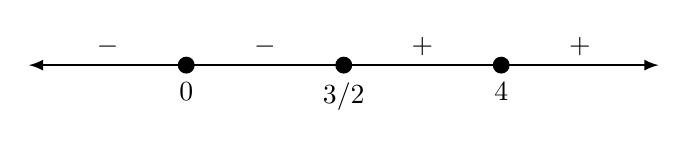
\begin{tikzpicture}[>=latex]
  \draw [thick, <->] (-4,0) -- (4,0);
  \draw [fill] (-2,0) circle [radius =.1];
  \draw [fill] (0,0) circle [radius =.1];
  \draw [fill] (2,0) circle [radius =.1];
  \node at (-3,0) [above] {$-$};
  \node at (-1,0) [above] {$-$};
  \node at (1,0) [above] {$+$};
  \node at (3,0) [above] {$+$};
  \node at (-2,-0.1) [below] {$0$};
  \node at (0,-0.1) [below] {$3/2$};
  \node at (2,-0.1) [below] {$4$};
  \end{tikzpicture}
\end{center}
   
   \item The intervals on which $f$ is increasing or decreasing.
   
   \medskip
   
From the sign diagram above, we see that $f$ is increasing on $(3/2,\infty)$ and decreasing on $(-\infty,3/2)$.

\medskip
   
   \item The coordinates of any local maxima or minima.

\medskip

  On our sign diagram, the only place where $f'$ changes sign is when $x=3/2$, where it changes from negative to positive, so we have a local minimum at this point. We find that $f(3/2)=(\frac32)^3(-\frac52)^5=-\frac{3^3\cdot 5^5}{2^8}$, so our local minimum is at $(3/2, -3^3\cdot 5^5/2^8)$.
   \end{enumerate}
   

   
   
  \end{enumerate}
\end{document}